\section{Overview of mapping problem and CyPhyHouse}
\label{sec:overview}

We first give an overview of the mapping problem, and the CyPhyHouse toolchain which we use to approach its solution. The features of the programming language $\lgname$ provided by CyPhyHouse enable us to design a succinct application for this problem, and set up terminology and formalization to aid in a correctness analysis. We also discuss at a high level, the features of CyPhyHouse toolchain that enable us to simulate and test this application for a multi-robot system under various deployment scenarios.

\subsection{Mapping problem }
\sayan{
Informally, the problem requires a set of robots to collaboratively mark the position of static \emph{obstacles} within a given area $D$, which any robot should avoid while moving in $D$.The key difference between distributed SLAM and this application is that we assume that the robots know their \emph{global coordinates} within the area of deployment. They are only attempting to map the static obstacles within this area. We currently assume that the only sensors available for sensing obstacles are LIDAR based, and the robots are constrained to move in a 2-D space.
}

\subsection{\dmap Application}

\reffig{flowmap1} shows a simple idea for solving the mapping problem problem for each robot, and \reffig{mapapp} shows our solution to $\dmap$ written using $\lgname$, a high level language with native support for multi-robot systems designed to interact with a physical environment. The design of solution to the mapping problem in \reffig{flowmap1} captures an occupancy map of the 2D space in a variable $\gmap$. \reffig{flowmap}. The variable $\lmap$ is a local mapping constructed by each robot $i$ using sensors, and information from other robots shared via $\gmap$. The robot first updates its $\lmap$ from $\gmap$, which stores the currently computed occupancy map \emph{by all robots}.  The robot then picks a new point in the grid known to be unoccupied in its $\lmap$ and follows a path ($\mathit{Motion.Path}$) moving only over grid rectangles known to be unoccupied by its $\lmap$. While the robot hasn't reached the target rectangle, it keeps updating its $\lmap$ with sensed data (occupied and unoccupied grid points). When it reaches the target, it updates the $\gmap$ with new data from its $\lmap$.


\begin{figure}[!htbp]
    \centering
    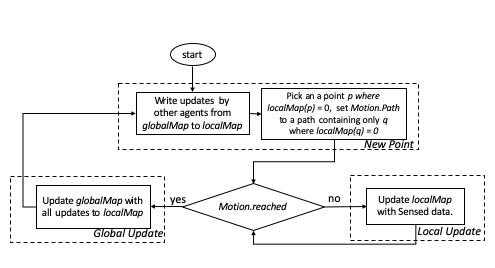
\includegraphics[width=\linewidth]{figs/map_flowchart.png}
    \caption{Flowchart for a simple solution to 2D distributed mapping problem\vspace{-2mm}}
    \label{fig:flowmap1}
\end{figure}

The $\lgname$ program corresponding to this solution has three \emph{events}: \emph{NewPoint, LUpdate, GUpdate}. Each robot in the system runs an instance of the \emph{same} program. At runtime, the $\lgname$ program executes within the runtime system of a single robot, or a collection of programs execute on different robots. The $\lgname$ language semantics ensures that the execution of the program in the distributed system occurs in \emph{rounds} of duration $\delta$. In each round, each robot executes the statements in the effect(\textbf{eff}) of at most one \emph{enabled} event : an event whose precondition(\textbf(pre)) is satisfied. If no event is enabled, the robot does nothing. Before the next round of execution, the robot may continue to interact with the physical environment as directed by its controllers. The $\lgname$ semantics imposes a synchronous model of execution for $\lgname$ programs for multi-robot systems and its implementation in CyPhyHouse toolchain ensures that this schedule is maintained by the multi-robot system executing the $\lgname$ program, despite potentially imprecise synchronization of local clocks.

\begin{figure}[!htbp]
    \noindent
    \begin{mdframed}

        \begin{center}
            \scriptsize
            \two{0.4}{0.6}
            {\lstinputlisting[language=xyzNums,firstline=1,lastline=21,frame=none]{code/mapapp.tex}}
            {\lstinputlisting[language=xyzNums,firstline=22,frame=none,firstnumber=22]{code/mapapp.tex}}
        \end{center}
    \end{mdframed}

    \caption{$\lgname$ code for robot $i$ for the 2D distributed mapping application. \vspace{-5mm}}
    \label{fig:mapapp}
\end{figure}


$\lgname$ provides \emph{shared} variables to allow robots within a system to communicate with each other. An \emph{allwrite} variable is a shared variable which all robots can read from and write to. The shared \emph{allwrite} variable $\gmap$ is used to construct a shared map of obstacles within the domain $D$, and has type $\mathit{GridMap}$, which is a 2-D array representing a grid over $D$. The \emph{local} variable $\lmap$ represents each robot's \emph{local} knowledge of the domain $D$, and has the same type as $D$. A robot executing the \emph{NewPoint} event, first updates a \emph{local variable} $\lmap$ from the shared variable $\gmap$, using a combination operator $\oplus$, described in more detail in \refsect{prelims}. $\lgname$ allows the user to use library functions, like the $\mathit{findPath}$ function, which uses a path planner to find a path to a point while avoiding a set of \emph{obstacles}. The point is picked using the $\mathit{pickFrontierPos}$ function which is a user defined function implemented in $\lgname$. The details of the path planner, and how the point is picked are discussed in and \refsect{prelims} \refsect{experiments}.

%\begin{itemize}
%    \item Multiple sensors
%    \item Sampled sensing : sensed over time.
%    \item Coordination using shared variables.
%    \item Mutual exclusion.
%\end{itemize}
% language features - what main "issue" each feature addresses .



 The program and the controller interact with each other through \emph{sensor} and \emph{actuator} ports. A $\lgname$ program can have multiple \emph{modules} providing different sensor and actuator ports. The program reads the sensor ports, reads and writes to program variables, and writes to actuator ports. The actuator ports of different modules can be used to provide input to the controller, which drives the underlying physical plant. In $\dmap$, there are two modules \emph{Motion} and \emph{Lidar} which provide interfaces to different sensors and actuators on the robot. The $\mathit{Lidar.ldata}$ sensor module is used to read the LIDAR scan of the actual robot. In the \emph{NewPoint} event, the controller driving the robot directs it along a path set at the actuator port $\mathit{Motion.path}$. The sensor port $\mathit{Motion.psn}$ gives the position of the robot (in a fixed coordinate system) and $\mathit{Motion.reached}$ indicates whether the controller is active or inactive.

In the design of the $\dmap$ application, we employ the use of \emph{sampled} sensors, which is essentially a sequence of timestamped sensor readings between rounds. The \emph{LUpdate} event can occur while each robot is traversing a path and hasn't reached the final destination, during which the robot uses a sampled sensor reading of the positions $\mathit{Motion.trace}$, of type $\mathit{PosStamped}[]$, which denotes an array of timestamped positions; and a sampled sensor reading of LIDAR scans $\mathit{Lidar.ldata}$ of type $\mathit{ScanStamped}$, which denotes an array of timestamped LIDAR scans. These sampled sensor readings are then synchronized to associate a LIDAR scan with a position.


Mutual exclusion is an essential feature required in a distribtued system with shared variables. The robot updates the shared variable $\gmap$ in the event \emph{GUpdate} using the value of its $\lmap$, which may have been updated with newly detected obstacles

%Also, should
The robot also has access to two system-level \emph{constant} parameters (a) a unique integer identifier $\myuin$ for itself and (b) a list $\UINS$ of identifiers of all participating robots\footnote{Our current system implementation assumes that the set of possible participating robots is known, but this assumption can be relaxed on a per application basis.}


\section{Koord Software Stack}
\label{sec:software}



\subsection{Formal semantics of Koord}
\label{sec:semantics}

The (distributed) system of robots  executing the \dmap application written in $\lgname$ can be viewed as a nondeterministic, state machine automaton~\cite{TIOAmon, Mitra07PhD}. The detailed statement-level semantics of $\lgname$ has been developed in the $\mathbb{K}$ framework and will appear elsewhere. For the purpose of the analysis here, we briefly describe the ``big-step'' semantics of Koord which allows all the statements in an event of a single robot to be executed as an instantaneous transition.

Suppose we have $N$ robots in the system each executing the same Koord application program. As mentioned earlier Koord middleware enforces a synchronous  \emph{round-by-round} execution, where each round lasts for $\delta$ time, where $\delta >0$ is a platform specific execution parameter.
%
In each round, each robot performs an  event.
The state update performed by a single robot executing an  event is modeled as an  transition of the state machine updating the program variables, however,  different events executed by the different robots may interleave. In between the events of successive rounds, the program variables remain constant, but {\em all\/} the \sayan{sensor and actuator variables} of all the robots  change continuously with time.  These are modeled as the $\delta$-transitions that advance time as well as the \sayan{sensor and actuator variables}.

%
Let the set of all program variables in the $\lgname$ application be $\Var$, and the set of all the sensor and actuator ports be $\mathit{Port}$. Let $\mathit{Event}_i$ be the set of events for the program for agent $i$.

%
The sets of variables and ports of an individual robot $i$ are denoted by $\Var_i$ and  $\mathit{Port}_i$.
%
A {\em valuation\/} of $\Var \cup \Port$ maps the names of the variables and ports to their types.
We denote valuations using boldface letter like $\vs, \vs_1, \vs'$, etc.
%
Given a valuation $\vs$, the value of a subset of  variables (or ports) $X$ is denoted by $\vs.X$. For example, the  valuation of all the variables of robot $i$ is $\vs.\Var_i$.
%
%
In the $\dmap$ $\lgname$ application,
\begin{inparaenum}
\item $\Var = \left\{ \gmap, \lmap, \mathit{newPoint}, \mathit{pscan}, \mathit{obstacles} \right\}$
\item $\Port = \left\{\mathit{ldata}, \mathit{trace}, \mathit{pos}, \mathit{trace}, \mathit{reached}, \mathit{target} \right\}$. \footnote{The syntax of $\lgname$ requires each \emph{actuator} and \emph{sensor} variable $v$ defined in a module $M$ to be referred to as $M.v$.}
\item For each robot $i$, $\mathit{Event}_i = \left\{ \mathit{NewPoint}, \mathit{LUpdate}, \mathit{GUpdate}\right\}$
\end{inparaenum}
%
%values that the variables can take is $\Val$, the \emph{state} of a robot $i$ is a tuple $$s_i = ( M, cp), \mbox{ where}$$
%
For the purpose of this paper, we define the  semantics of the overall system with $N$ robots as discrete transition system $\A = (C, C_0, A, \D)$,
where
(1) $C$ is the set of valuations of all the variables $\Var$ and all the ports $\mathit{Port}$ for each robot,
(2) $C_0 \subseteq Q$ is the set of initial values of the variables and port for each robot. All variables and ports have to be initialized,
(3) $A = \{\delta\} \cup \left( \cup_{i \in [N]} \mathit{Events}_i \right)$ is the set of transition labels, and
(4) $D \subseteq C \times A \times C$ is a set of transitions. The state of the system is a valuation $\vs \in C$. There are two types of transitions, namely:
\begin{enumerate}
	\item {\em event transition}: Any $a \in \Event_i$ for some $i \in [N]$, and  given $\vs, \vs'\in C$,   $(\vs,a,\vs') \in \D$ iff (i) $\vs'.\Var_i$ is obtained by applying the transition relation of $a$ to $\vs.\Var_i$, where $\vs.\Var_i$ refers to the mapping of all variables of robot $i$ to their values in the state $\vs$.
		(ii) For all $j \neq i$,
		$\vs'.\Var_j = \vs.\Var_j$.
	\item {\em $\delta$-transition}: $a = \delta$, and $(\vs,a,\vs') \in \D$ iff $\vs'.\Var = \vs.\Var$.
\end{enumerate}
\rg{We assume that the event transitions are computational steps, and take zero logical time, whereas the $\delta$-transitions denote the evolution of the sensor and the actuator ports with time, and take $\delta$ time.}\fTBD{restate in assumptions}.
\sayan{This formalization allows the ports to behave arbitrarily over $\delta$-transitions. In order to establish invariant properties of applications, therefore, we will need to constrain the behavior of the sensor and actuator ports with additional assumptions.
}


A \emph{program step} is a sequence  $\vs_0 , a_0,  \vs_1, a_1, \ldots  ,a_N \vs_N$ of length $N$, where $(\vs_i , a , \vs_{i+1}) \in D$ is an event transition. Given a program step $\ps = \vs_0 , a_0,  \vs_1, a_1, \ldots  ,a_N \vs_N$, $\ps[i]$ refers to the state $\vs_i$.
An \emph{execution} of a system is an alternating sequence of program steps and $\delta$-transitions $\ps_0, d_0 , \ps_1, d_1, \ldots$ where
\begin{itemize}
\item $\ps_i$ is a program step and $d_i$ is a $\delta$-transition,
\item $\ps_0$ is a program step $\vs_0, a_0, \vs_1, \ldots ,a_N, \vs_N $  where $\vs_0 \in C_0$,
\item Given a $\delta$-transition $d_i = (\vs, a, \vs')$, and its preceding program step $\ps_i$,  $\ps_i[N] = \vs $
\end{itemize}
%
%of each robot evolve to the 	controllers driving the robot according to the actuators that may have been set in the event. The program and sensor variables of the robot can be seen as the state variables for each robot.


%\begin{enumerate}
%    \item $M : \Var \mapsto \Val$ is the mapping of all program variables in the application known by the robot to their values.
%    \item $cp : \Var \mapsto \Val$ is the mapping of actuator and sensor variables to their values.
%\end{enumerate}
%The components of the tuple $s_i$ are accessed using the dot $`.'$ notation, for instance, $s_i.M$, etc. The value of a program variable $v$ at a state $s_i$ is denoted by $s_i.M.v$.

We define the set of reachable states of a system $\A$ , $\Reach(\A) = \{c \mathit c \in C_0 \vee \exists c^\prime \in \Reach(\A), (c^\prime, a, c) \in \D \}$. A predicate $\mathcal{P} : C \mapsto \mathbb{B}$ is an \emph{invariant} of the $\A$, if $\forall q \in \Reach(\A), \mathcal{P} = \mathit{True}$.

\subsection{Runtime system}



To run a $\lgname$ program (hardware or simulation), the user has to provide a configuration file, with
\begin{inparaenum}
    \item the number of robots,
    \item in case of simulation, the initial positions of the robots and the length of the simulation and
    \item in case of hardware deployment their IP addresses,
    and the localization system.
\end{inparaenum}



\subsection{Simulator}
\subsubsection{gazebo environment}
\subsubsection{car model}
\subsubsection{lidar}
\subsubsection{positioning}
\subsubsection{sampled sensing}
\subsubsection{synchronization issues}


